% !TEX root = ../../thesis.tex

\documentclass[../../thesis.tex]{subfiles}
 
\begin{document}

In this chapter, we experiment our solvers and discuss the results. 

\section{Benchmark process}

Our benchmark API takes an options structure (\autoref{benchmark:options}).
The arrays \texttt{T}, \texttt{D} and \texttt{W} determines the sizes of the instances. The benchmark runner 
will create instances with a combinations of those parameters. For example, with the values in \autoref{benchmark:options},
the benchmark runner will create 6 instances with the sizes: $(5, 30, 100)$, $(5, 50, 100)$, $(5, 30, 200)$, $(5, 50, 200)$, $(5, 30, 300)$ and $(5, 50, 300)$ with the 
three values being $(T, D, W)$.

\begin{lstlisting}[style=scalaStyle,label={benchmark:options},caption={Benchmark options},captionpos=b]
trait BenchmarkOptions {
  val solutionLimit: Int = Int.MaxValue
  val timeLimit: Int = 20
  val repeat: Int = 1
  val dryRun: Int = 1
  val T: Array[Int] = Array(5)
  val D: Array[Int] = Array(30, 50)
  val W: Array[Int] = Array(100, 200, 300)
  val probabilities: Map[String, Double] = Map()
  val seed: Long = -1L
}
\end{lstlisting}

We can specify a solution limit as well as a time limit. We can also repeat our benchmark and takes 
the average of results. We can also have dry runs to warm up the JVM (Java Virtual Machine) and a seed to have reproducible benchmarks. Finally,
we can specify the probabilities for our instances as explained in \autoref{section:instance-gen}.

Our benchmark runner has a function \texttt{run} that takes a name (e.g. solver name, serie name, etc), and a solving function 
which takes a generic model and returns a pair with the time spent in milliseconds and the objective value respectively.

\begin{lstlisting}[style=scalaStyle,label={benchmark:run},caption={Benchmark run function},captionpos=b]
class BenchmarkRunner(val options: BenchmarkOptions) {
  def run (
    name: String, 
    solve: VillageOneModel => (Long, Int)
  ): (BenchmarkSerie, BenchmarkSerie)
}
\end{lstlisting}

This functions returns a pair of benchmark series: one serie for the time values and one serie for the objective values.
The \texttt{BenchmarkSerie} class is simply a class that takes a name and a list of benchmark measurements (i.e. mean, standard deviation, min and max).

This implementation allows us to create a variety of benchmark by simply changing the \texttt{solve} function.


\section{Constraint Programming}

\subsection{Comparison between heuristics}

We talked in \autoref{section:cpmodel} about our custom heuristic called Most Available Heuristic.
We now compare the performance of this heuristic with standard heuristic like the \texttt{max-value} heuristic.
We also compare the variable heuristics used in addition to our aforementioned heuristic.

\subsubsection{\texttt{mostavailable} \& \texttt{max-value}}

The \texttt{max-value} heuristic is a value heuristic that takes the maximum value in the domain of a selected variable during the search.
It's one of the simplest value heuristic that can be implemented but unfortunately does not offer great performances.

\autoref{experiments:heuristic1} shows the objective ratio between the implemented custom \textit{Most Available} Heuristic and a standard 
\textit{First Fail} variable heuristic with the \texttt{max-value} value heuristic after the first solution.
The two heuristics were tested on 72 instances of various sizes from small to big instances.
The performance profile shows a clear gain of about $2$ to $3.4$ for our custom heuristic.


\begin{figure}
  \centering
  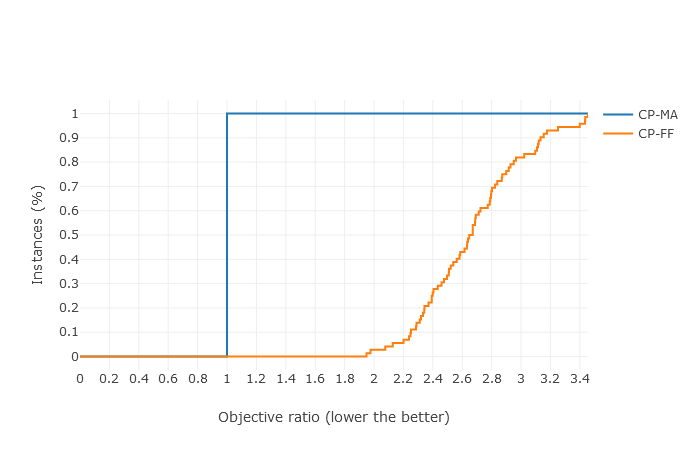
\includegraphics[scale=0.55]{experiments/heuristic.png}
  \caption{Most Available and First Fail heuristics [72 instances/first solution].}
  \label{experiments:heuristic1}
\end{figure}


\subsubsection{\texttt{mostavailable} \& dynamic \texttt{mostavailable}}

We also discussed in \autoref{section:cpmodel} an improvement based on the \texttt{mostavailable} static ordering
where we ordered dynamically the most available worker at each value selection.

\autoref{experiments:heuristic2} shows the performance profile of the dynamic \& static most available heuristics.
This benchmark was performed on 486 instances for a duration of 15 seconds each.

TODO: performance analysis



As our dynamic value heuristic outperforms every other tested heuristic, we will assume for the rest of this chapter 
that the value heuristic for the Constraint Programming solver is the dynamic \texttt{mostavailable}.

%We can see a slight 
%improvement of about 10\% to 60\% for approximately 90\% of instances and as much as 2 to 4 times an improvement for the remaining instances. 


\begin{figure}
  \centering
  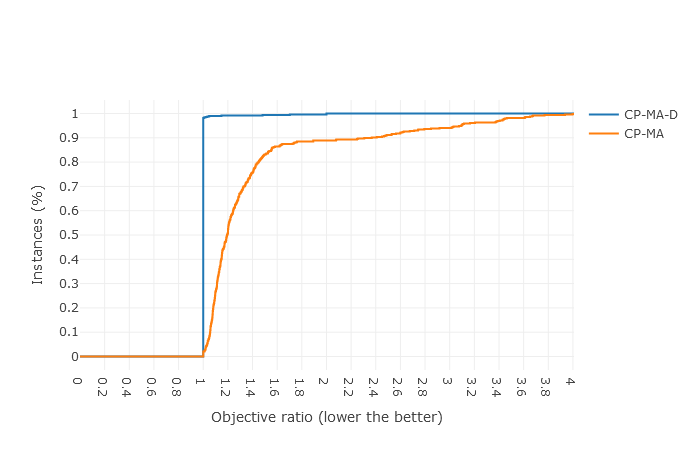
\includegraphics[scale=0.55]{experiments/static-dynamic-heuristic.png}
  \caption{Most Available: static and dynamic [486 instances/15s].}
  \label{experiments:heuristic2}
\end{figure}


\subsubsection{Max Degree \& Min Size}

In addition to our Most Available heuristic, we use a variation of the \texttt{maxdegree} heuristic. 
This heuristic is a first-fail variable heuristic that selects the most constrained unbound variable. However,
as stated in our model in \autoref{section:cpmodel}, skills are not represented with constraints but instead values 
are removed from the domain at initialization. To express skills as part of the max degree, we simply add the number of 
skills required by a variable to the degree of that variable. The \texttt{minsize} heuristic is also a first-fail variable heuristic which 
selects the variable with minimum domain size.

TODO FIGURE + PERF ANALYSIS 


\subsubsection{Max Degree \& Conflict Ordering Search}

Conflict Ordering Search (COS) \cite{Gay:COS} is a variable ordering heuristic that 
reorders variables based on the number of conflicts that happen during the search.
It is a variant to the Last Conflict heuristic that selects the variable which caused the last conflict first.
COS was shown to be the most performant on scheduling problems.


TODO: FIGURE + PERF ANALYSIS

\begin{figure}
  \centering
  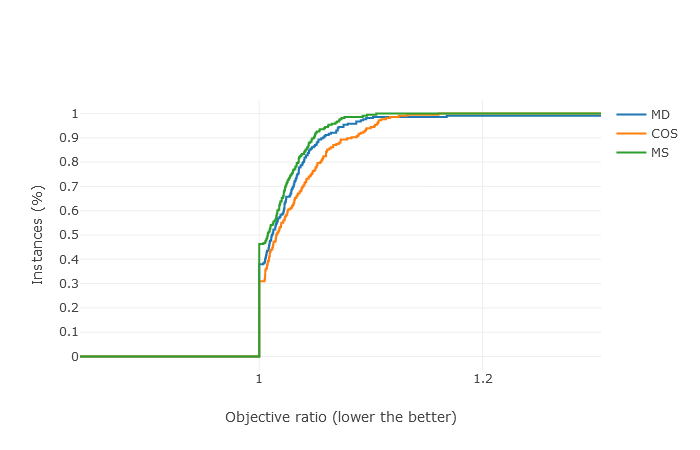
\includegraphics[scale=0.55]{experiments/cos-md-ms.png}
  \caption{COS, Max Degree and Min Size heuristics [216 instances/30s].}
  \label{experiments:heuristics:3}
\end{figure}


\subsection{Comparison between searches}


As stated in \autoref{chapter:sota} and \autoref{section:cpmodel}, LNS is used to expand the exploration
of the search tree. We now compare our solver with the use of LNS and without. We also compare multiple 
relaxations method.


\subsubsection{Standard Search \& LNS}


% \begin{figure}
%   \centering
%   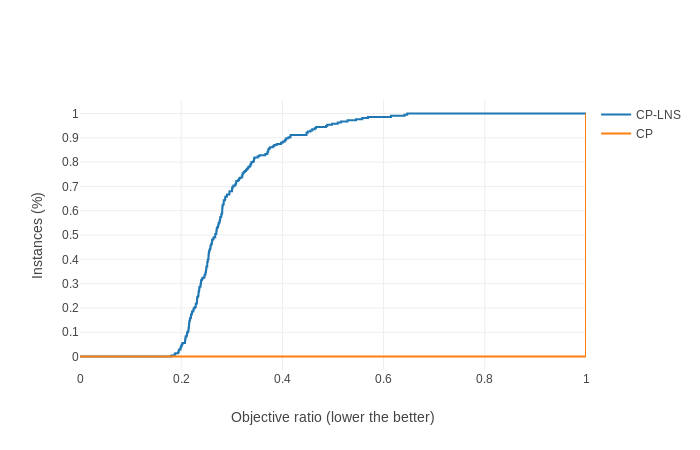
\includegraphics[scale=0.55]{experiments/lns.png}
%   \caption{CP with and without Large Neighborhood Search [216 instances/30s].}
%   \label{experiments:lns}
% \end{figure}

\begin{figure}
  \centering
  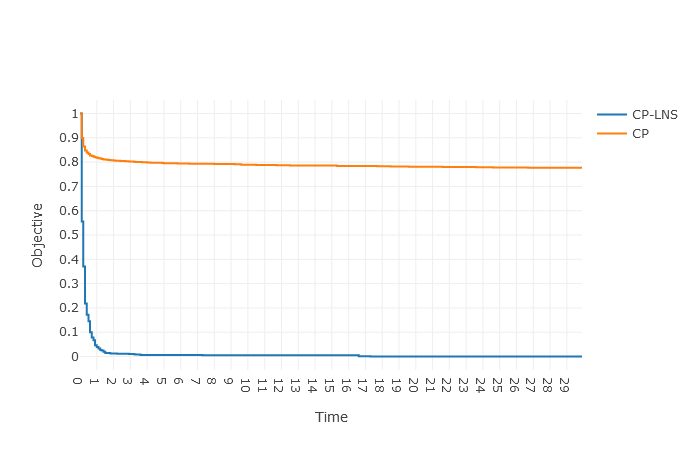
\includegraphics[scale=0.55]{experiments/lns-oot.png}
  \caption{CP with and without Large Neighborhood Search [216 instances/3s].}
  \label{experiments:lns}
\end{figure}


TODO: FIGURE + PERF ANALYSIS


\subsubsection{Random Relaxation \& Propagation Based Relaxation}

TODO: FIGURE + PERF ANALYSIS

\section{Comparison between solvers}

We now start by comparing different solvers together. \autoref{experiments:solvers:3} 
shows a performance profile generated from 216 instances of various sizes.
This benchmark was set to a time limit of 30s per instance. The baseline of this 
profile is the CP solver. We observe that the CP solver performs better than MIP in more than 80\% of instances.
However, we also tested the MIP solver by giving it a first solution obtained from CP, we can see that it slightly outperforms CP and MIP in 80\% of instances.

\begin{figure}
  \centering
  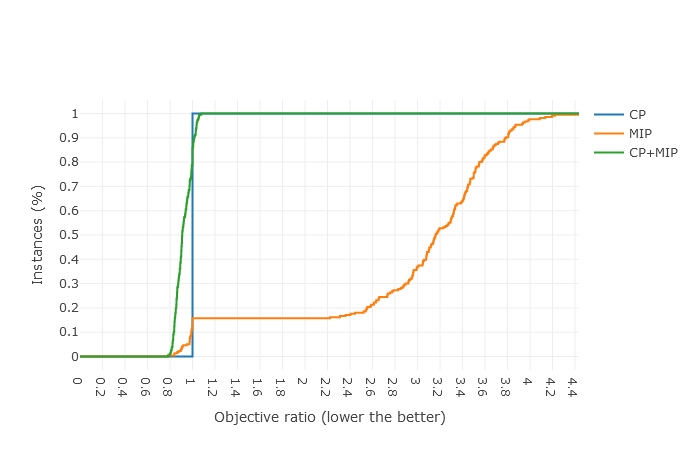
\includegraphics[scale=0.55]{experiments/solvers.png}
  \caption{CP, MIP and CP+MIP solvers [216 instances/30s].}
  \label{experiments:solvers:3}
\end{figure}


\begin{figure}
  \centering
  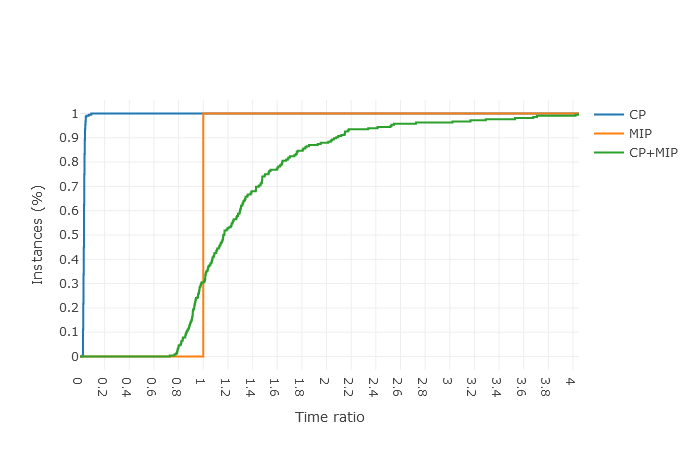
\includegraphics[scale=0.55]{experiments/time-first-sol.png}
  \caption{Time on first solution [216 instances/First solution].}
  \label{experiments:first-sol-time}
\end{figure}


\begin{figure}
  \centering
  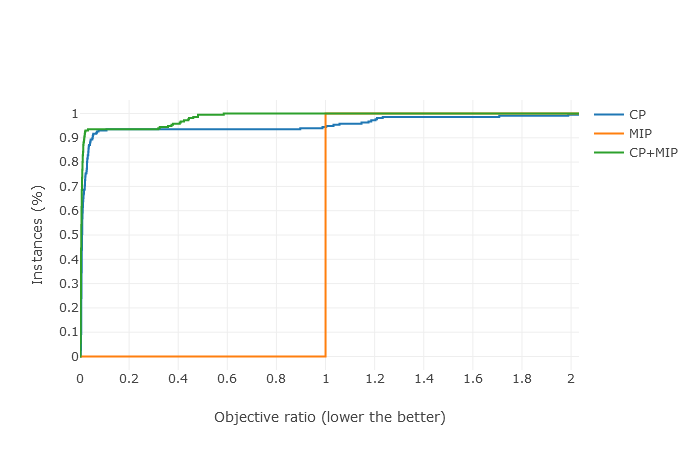
\includegraphics[scale=0.55]{experiments/obj-first-sol.png}
  \caption{Objective on first solution [216 instances/First solution].}
  \label{experiments:first-sol-obj}
\end{figure}




\end{document}

